\tab Putem avea conflicte in cazul cind dorim sa facem merge la 2 branchuri si unele
rinduri sunt diferite. In asa caz ne vin in ajutor un mergetool. Drept mergetool am ales
\textbf{kdiff3}. Pentru a seta kdiff3 ca mergetool default folosim comanda : 
\textbf{git config --global merge.tool kdiff3}
~\\
\tab In continuare vom lucra cu 2 branchuri - "master" si "nou". Vom crea in fiecare
branch cite un fisier "tomerge" continutul caruia va fi diferit.\\
~\\
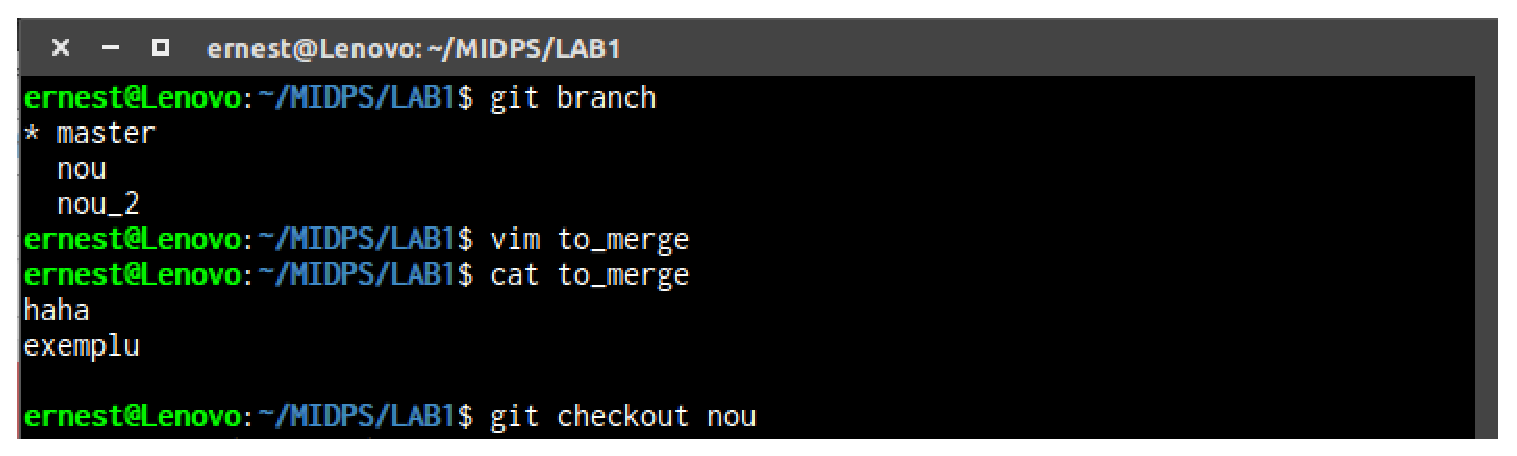
\includegraphics[width=\textwidth]{13.eps}\\
~\\
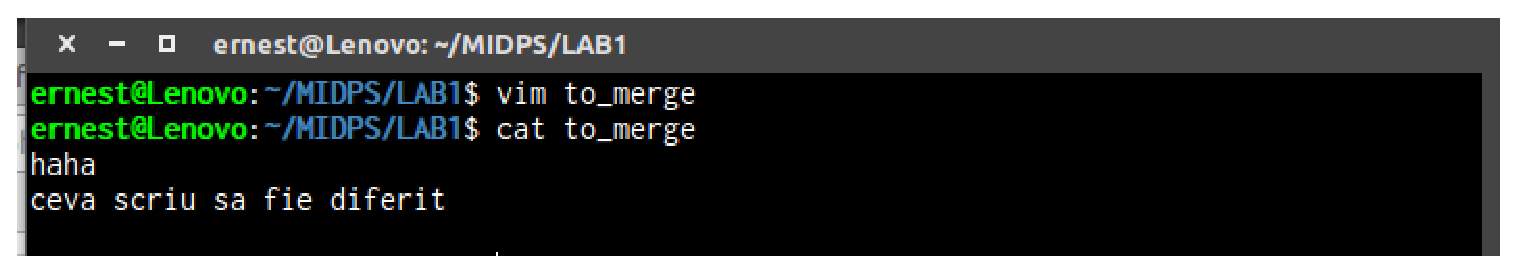
\includegraphics[width=\textwidth]{14.eps}\\
~\\
In continuare vom incerca sa facem merge si sa rezolvam acest conflict.\\
~\\
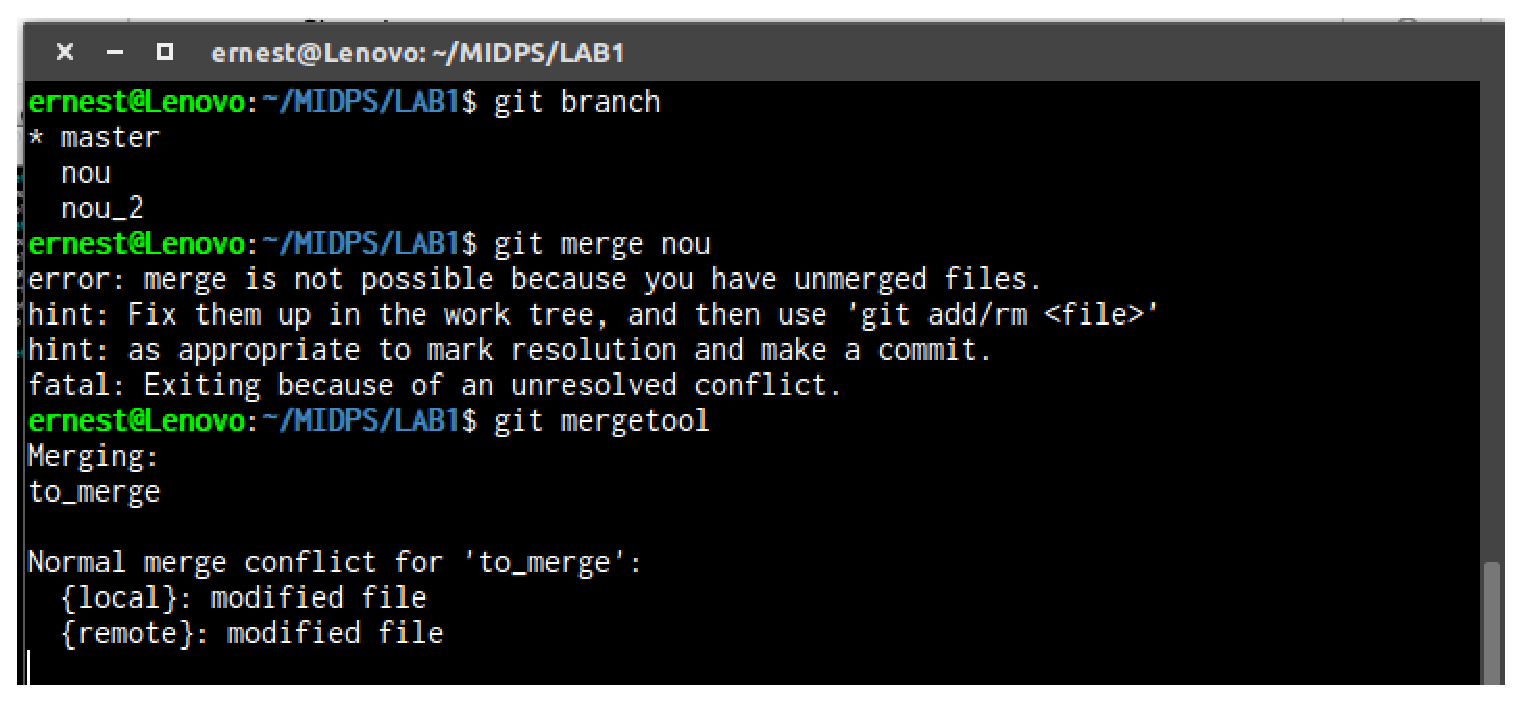
\includegraphics[width=\textwidth]{15.eps}\\
\clearpage
Dupa acest pas rezolvam conflictul cu ajutorul \textbf{kdiff3}. De exmplu eu 
am ales sa fac merge in felul urmator.\\
~\\
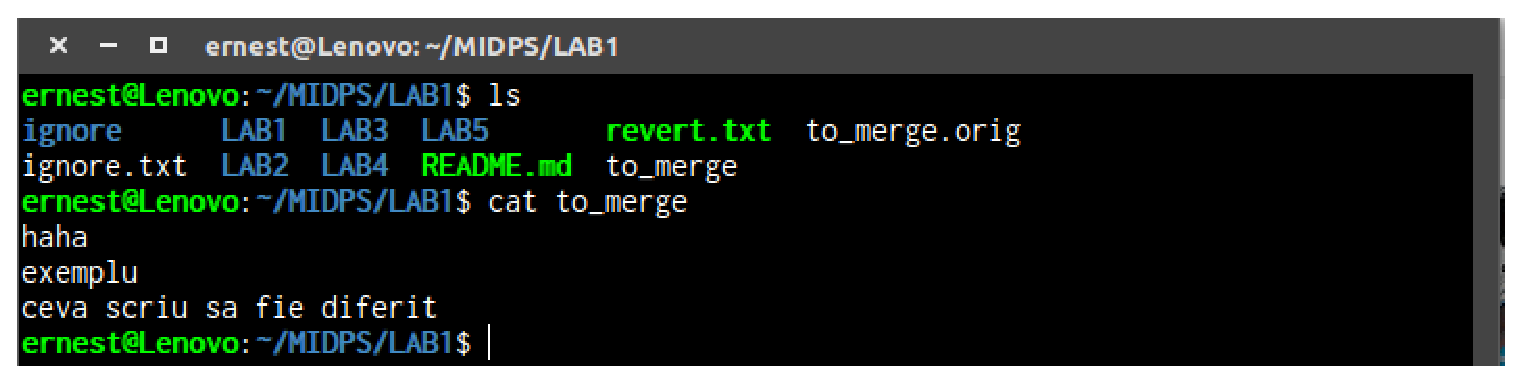
\includegraphics[width=\textwidth]{16.eps}\\
~\\
\textbf{Tagurile} sunt foarte comod de folosit si cu ajutorul lor putem face un track
eficient al versiunelor. Exemplu de tag.\\
\\
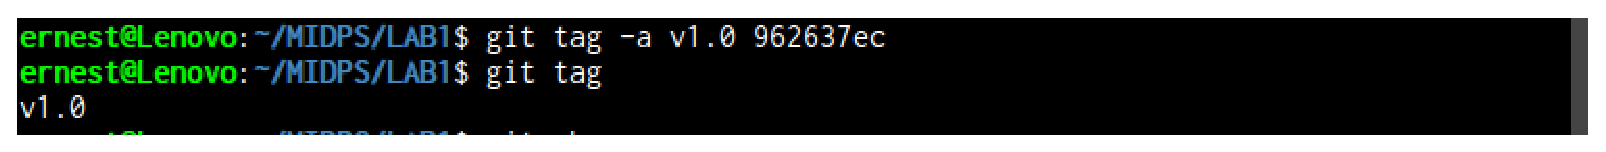
\includegraphics[width=\textwidth]{17.eps}\\
~\\
Dupa aceasta putem vedea usor o versiune taguita. Folosim comanda
\textbf{git show "tag"}\\
~\\
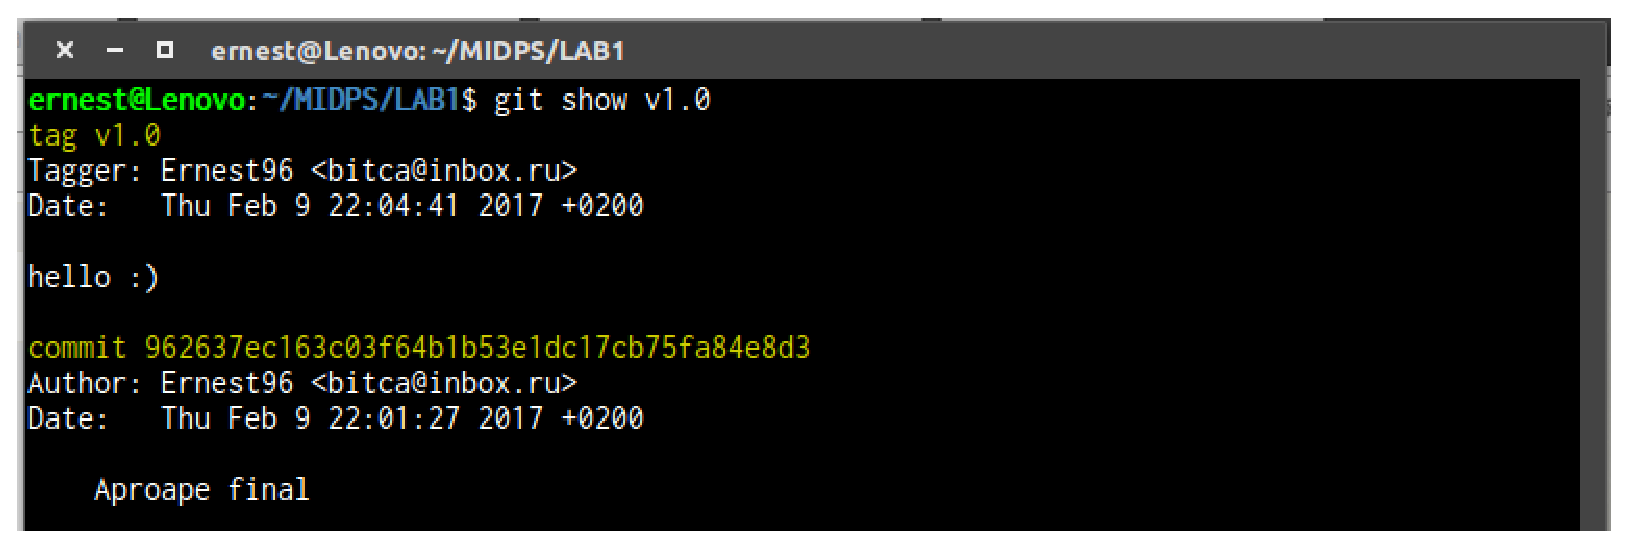
\includegraphics[width=\textwidth]{18.eps}\\
\clearpage
